\documentclass{standalone}
\usepackage{pgfplots}
\pgfplotsset{compat=newest}

\begin{document}
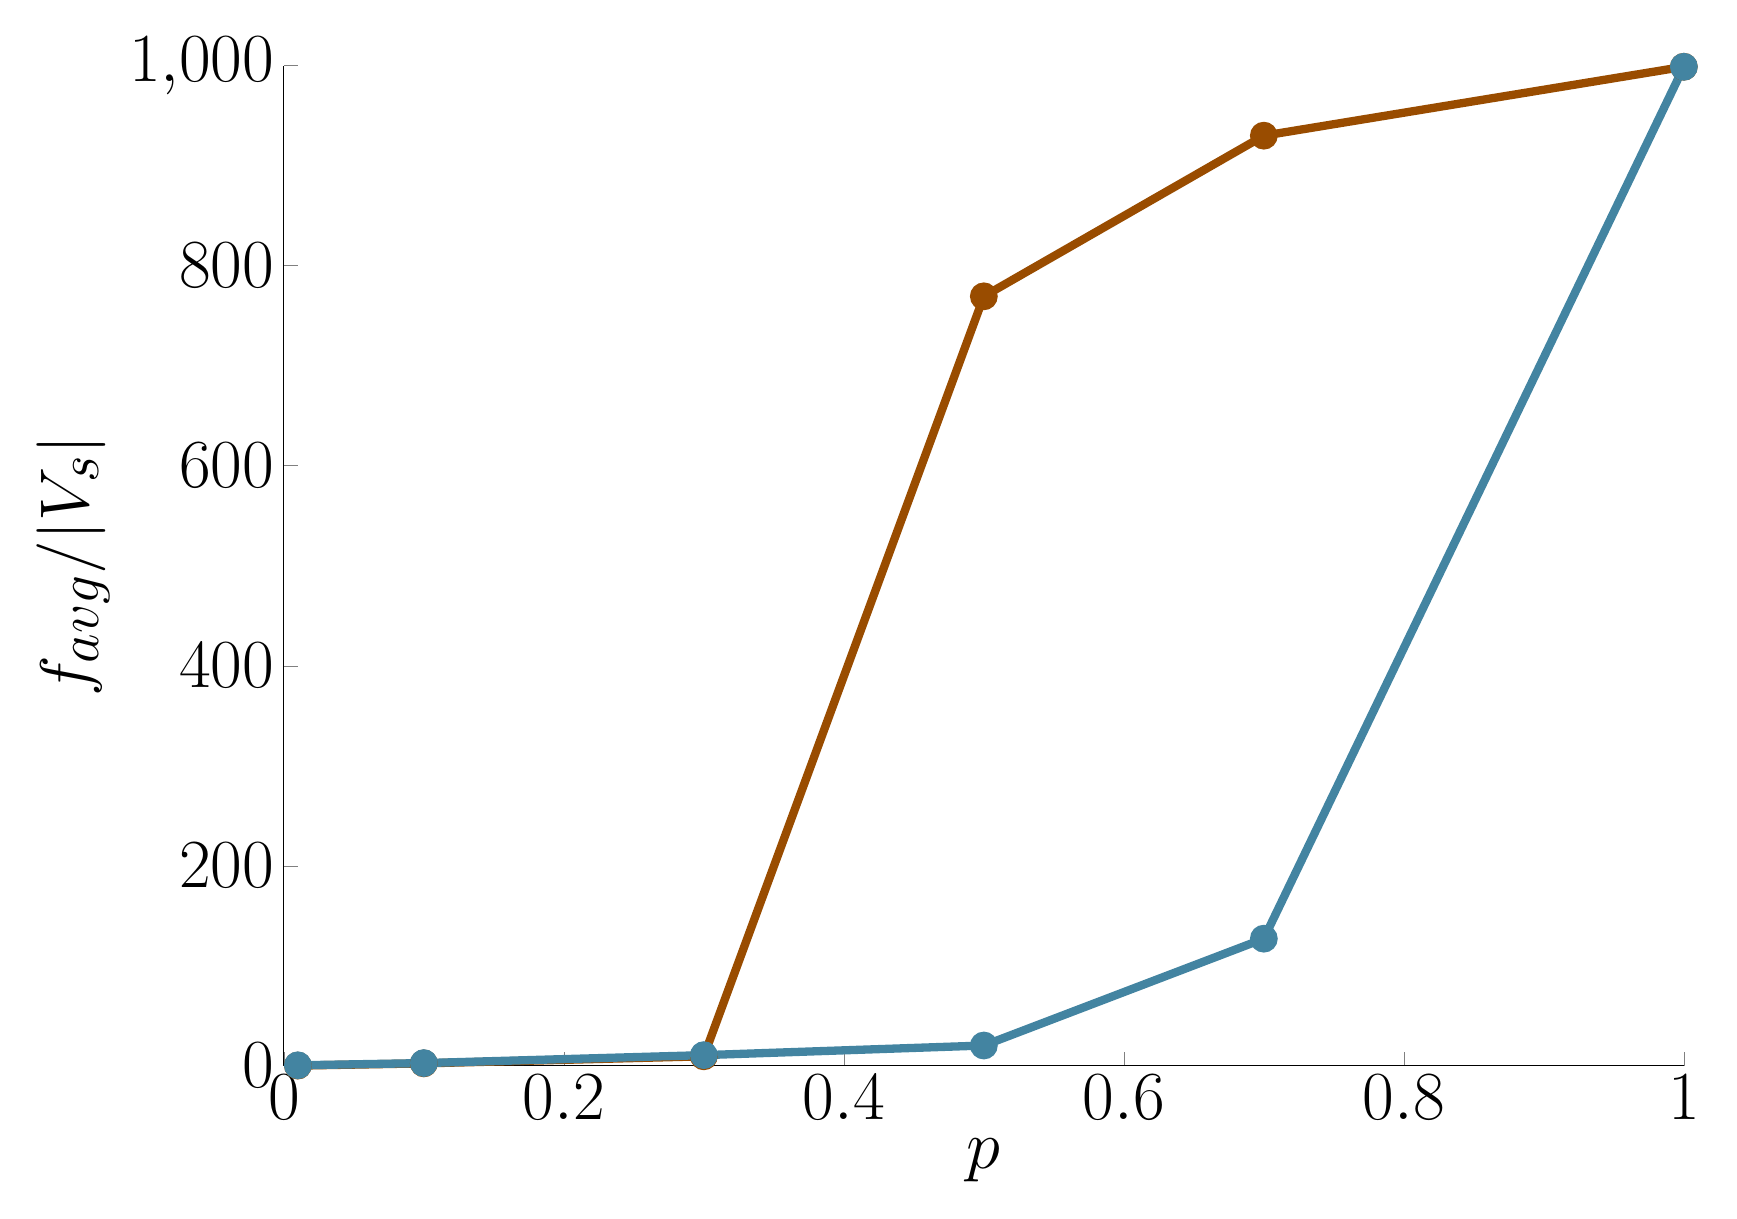
\begin{tikzpicture}

\begin{axis}[%
tick label style={font=\Huge},
label style={font=\Huge},
legend style={font=\Huge},
view={0}{90},
width=7in,
height=5in,
scale only axis,
xmin=0, xmax=1,
xtick={0, 0.2, 0.4, 0.6, 0.8, 1},
xlabel={$p$},
ymin=0, ymax=1000,
ytick={0, 200, 400, 600, 800, 1000},
ylabel={$f_{avg} / |V_s|$},
major tick length=5pt,
axis lines*=left,
legend cell align=left,
clip=false]

\addplot [
mark=*,
mark size=3.5pt,
color=orange!60!black,
solid,
line width=3pt
]
coordinates{
(0.01,0.172)(0.1,2.414)(0.3,9.47)(0.5,769.45)(0.7,930.1)(1,999.0)
};

\addplot [
mark=*,
mark size=3.5pt,
color=cyan!60!black,
solid,
line width=3pt
]
coordinates{
(0.01,0.488098739496)(0.1,2.695)(0.3,10.641)(0.5,20.2682152543)(0.7,127.110315934)(1,999.0)
};

\end{axis}
\end{tikzpicture}
\end{document}
